\documentclass[12pt, aspectratio=43]{beamer} 

\input{package.tex} % 載入封包與文檔配置

% Title, Subtitle, Author, Institute, Date
\title[\textbf{Week 8 Report}]{Week 8 Report}
\author[Chen, Pin-Jui]{Chen, Pin-Jui}
\date{\today}

\begin{document}
	
	% Title page frame
	\begin{frame}
		\titlepage
	\end{frame}
	
	% Index

	
	\begin{frame}
		\tableofcontents[currentsection,]
	\end{frame}
	
	\section{Single-cell gene set analysis Methods}
	
	\begin{frame}
		The commonly used scGSA methods are based on
		\begin{enumerate}
			\item Ranking
			\item Aggregating gene expression
		\end{enumerate}
		These methods have several problems:
		\begin{enumerate}
			\item sensitive to gene set size
			\item sparsity
			\item poor reproducibility
		\end{enumerate}
		
	\end{frame}
	
	\begin{frame}{Existing Methods}
		The commonly used scGSA methods are based on
		\begin{enumerate}
			\item Ranking-bases
			\begin{enumerate}
				\item \textbf{ssGSEA} : calculated by the Kolmogorov–Smirnov-like random walk statistic
				\item \textbf{UCell} : calculates the Mann–Whitney U statistic
				\item \textbf{AUCell} : calculates the area under the curve (AUC) score among all ranked genes
				\item \textbf{JASMINE} : calculates the enrichment of the signature using the mean rank of the expressed genes, the proportion of expressed to nonexpressed genes and the proportion of expressed genes in the gene set
			\end{enumerate}
			
		\end{enumerate}
		
		
	\end{frame}
	
	
	\begin{frame}{Existing Methods}
		\begin{enumerate}
			\item Count-based
			\begin{enumerate}
				\item \textbf{AddModuleScore} : a function in Seurat package and calculates scores for individual cells by aggregating the expression levels of each gene set, which are then subtracted by the aggregated expression of control feature sets randomly selected as background
				\item \textbf{SCSE} : calculated as a sum of gene expression within gene sets divided by the sum of gene expression for each cell
			\end{enumerate}
		\end{enumerate}
	\end{frame}
	
	\section{scPS}
	
	\begin{frame}{scPS}
		\begin{align}
			scPS = \mu \times \sqrt{\sum^m_{i = 1}(s_i - s_{min})\times v_i}
		\end{align}
		$\mu$ is the mean gene expression of the gene set. \\
		$s_i$ is the unweighted principal component score (PC). \\
		$s_{min}$ is the minimum of the si among all the cells. \\
		$v_i$ is the percentage of variance explained by the PC. \\
		$m$ is the number of PCs at which 50$\%$ cumulative variance is explained.
	\end{frame}
	
	\begin{frame}{Result}
		scGSA methods for the comparative analysis
		\begin{enumerate}
			\item Effect of the \textbf{cell count} on scGSA performance
			\item Effect of \textbf{gene set size} on scGSA performance
			\item Effect of the \textbf{noise level} on scGSA performance
			\item Effect of the \textbf{condition-specific genes} on scGSA
			performance.
		\end{enumerate}
	\end{frame}
	
	\begin{frame}{zero inflation}
		Common "zero inflation" issues in single-cell RNA data:
		\begin{enumerate}
			\item Many genes show an expression level of 0 (this could be due to genuine lack of expression or technical dropout);
			\item PCA may be dominated by these zero values, causing false signals;
			\item Genes with low expression levels may be mistakenly identified as important variants.
		\end{enumerate}
		To address this issue, paper used \textbf{scImpute}. 
		\vskip 0.2cm
		ScImpute effectively reduces dropout rates in scRNA-seq data by employing a sophisticated model that combines \textbf{gamma and normal distributions}.
	\end{frame}
	
	\section{experiment setting}
	
	\begin{frame}{Gene set simulation}
		\begin{enumerate}
			\item Gene set size : 10 ~ 500
			\item Noise : 0, 20, 50, 80, 100$\%$
			\item Generate 100 Gene set for each
			\item Total 5,000 Gene set
		\end{enumerate}
	\end{frame}
	
	\begin{frame}{Data simulation and signal assignment}
		Sample sizes of 20, 50, 200 and 500 cells in each group.
		\vskip 0.2cm
		\textbf{Data}
		\begin{enumerate}
			\item Splatter simulated data (SSD) : generated using the Splatter package.
			\item real-world simulated data (RWSD) were generated using log-transformed publicly available data.
		\end{enumerate}
	\end{frame}
	
	\begin{frame}{Scenario}
		Gene expression ( treatment (20$\%$) > control )
		\begin{enumerate}
			\item scenario 1 : At least 50 densely expressed genes (90$\%$ SSD vs 75$\%$ RWSD)
			\item scenario 2 : Random choose 550 genes
		\end{enumerate}
		To evaluate the zero imputation effect
		\begin{enumerate}
			\item no gene received any signal in these scenarios
			\item scenario 3 : introduced 250 (∼2$\%$) more genes into the treatment group.
			\item scenario 4 : introduced 250 (∼2$\%$) more genes into the treatment group (sparse).
		\end{enumerate}
	\end{frame}
	
	\begin{frame}{Scenario}
		\begin{figure}[h!]
			\centering
			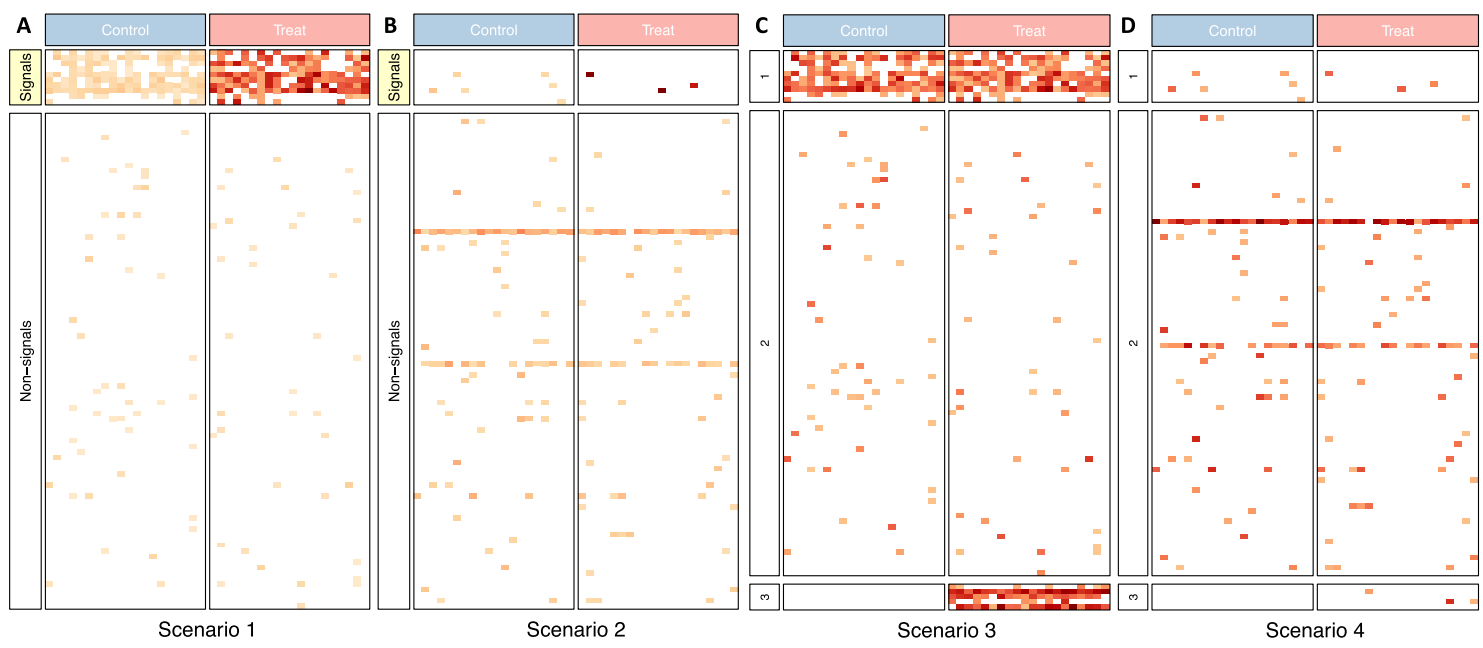
\includegraphics[width=\linewidth]{Figure/scenario.png}
		\end{figure}
	\end{frame}
	
	
	\section{Result}
	\begin{frame}{Recovery rate}
		Recovery rate:
		\begin{align}
			\dfrac{\text{Number of correctly identified gene sets}}{\text{Total number of simulated gene sets}}
		\end{align}
		Find Gene set
		\begin{itemize}
			\item Wilcoxon test
			\item FDR
			\item p-value < 0.05
		\end{itemize}
			
	\end{frame}
	
	\begin{frame}{Effect of the cell count on scGSA performance}
		%We measured the recovery rate of the gene sets consisting of 100 signal genes
		\begin{figure}[h!]
			\centering
			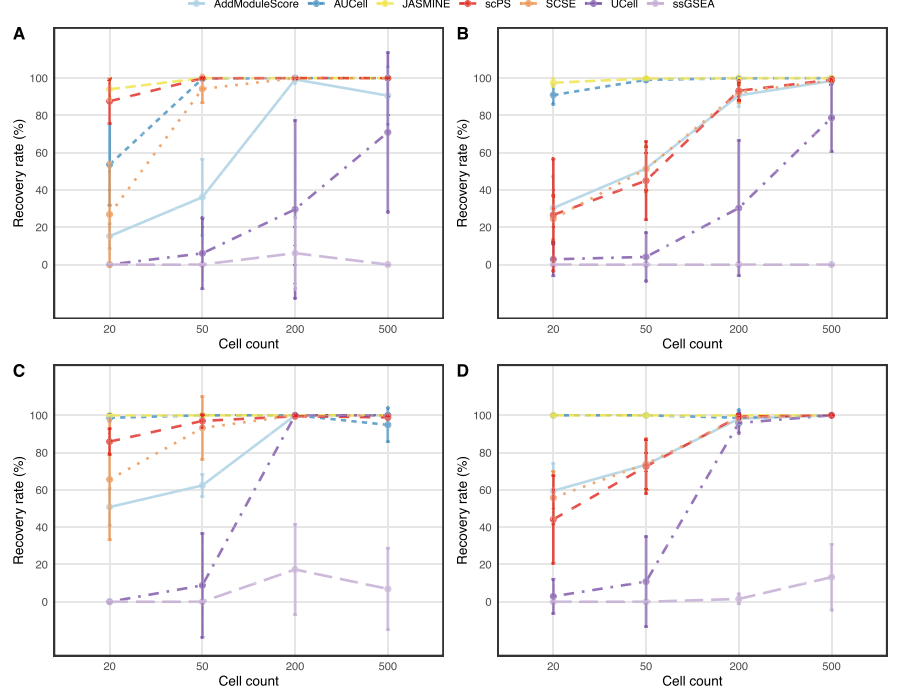
\includegraphics[width=0.9\linewidth]{Figure/cell.png}
		\end{figure}
	\end{frame}
	
	\begin{frame}{Effect of the cell count on scGSA performance}
		\begin{enumerate}
			\item AddModuleScore, SCSE and UCell improved as the number of cells increased in both scenarios
			\item UCell had a high standard deviation, attributable to the relatively high variability in the long tail of bottomranking genes.
			\item The results in RWSD were better than those in SSD, which had a higher signal-to-non-signal ratios (SNR) and relatively lower sparsity.
			\begin{figure}[h!]
				\centering
				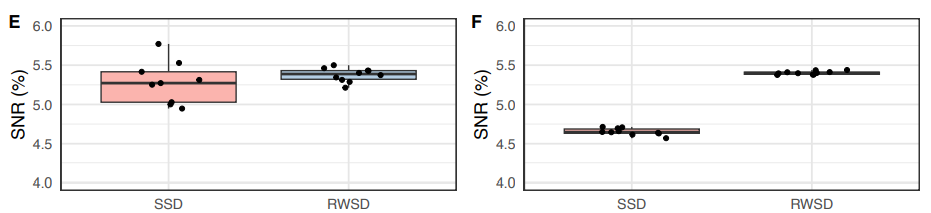
\includegraphics[width=\linewidth]{Figure/rwsd_ssd.png}
			\end{figure}
		\end{enumerate}
	\end{frame}
	
	\begin{frame}{Effect of gene set size on scGSA performance}
		%Fix 200 cells per group and gene sets with a noise level of 0$\%$
		\begin{figure}[h!]
			\centering
			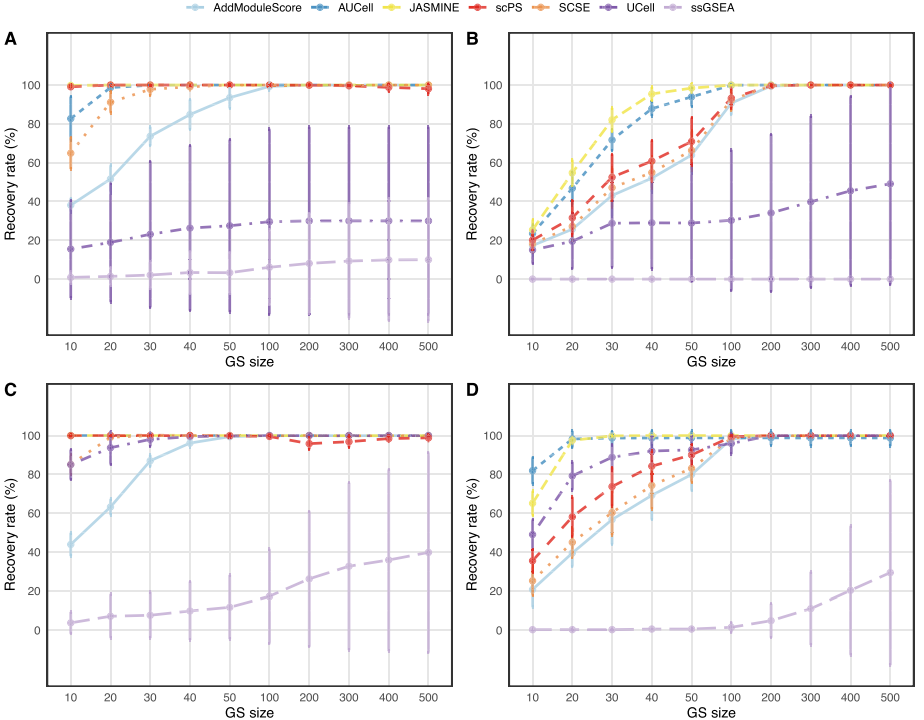
\includegraphics[width=0.9\linewidth]{Figure/GS.png}
		\end{figure}
	\end{frame}

	\begin{frame}{Effect of gene set size on scGSA performance}
		\begin{enumerate}
			\item In scenario 1, 2, all differentially expressed gene sets between sizes of 200 and 500 were identified by all methods except ssGSEA
			\item AddModuleScore performed well with a gene set size >50
			\item UCell and ssGSEA performed poorly across all gene set sizes in SSD.
			\item AUCell performed better when the data had a higher SNR and lower dropout rate upon zero imputation because AUCell randomly assigned ranks to genes with the same expression, leading to skewed results. 
			\item JASMINE considers the mean rank of the gene set and the ratio of expressed and unexpressed genes within or outside the gene set, which leads to a higher recovery rate when the data has a higher dropout rate, such as in single-cell datasets (SSD).
		\end{enumerate}
	\end{frame}
	
	
	\begin{frame}{Effect of the noise level on scGSA performance}
		\begin{figure}[h!]
			\centering
			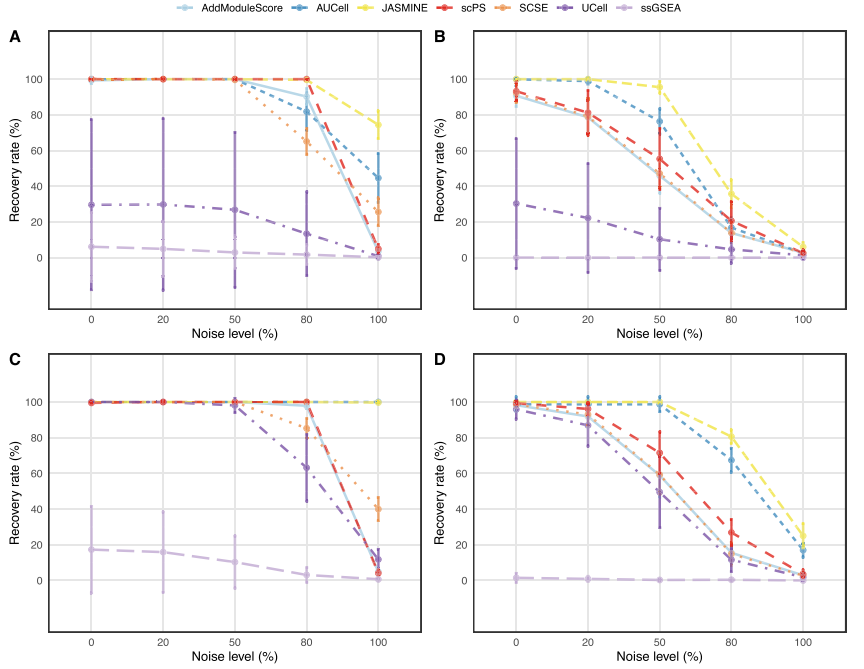
\includegraphics[width=0.9\linewidth]{Figure/noise.png}
		\end{figure}
	\end{frame}
	
	\begin{frame}{Zero-impute data}
		\begin{figure}[h!]
			\centering
			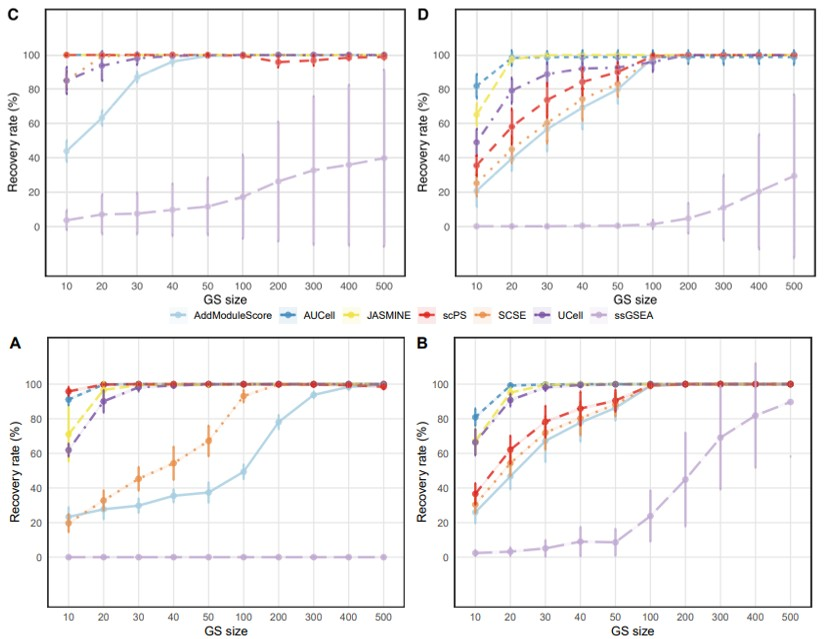
\includegraphics[width=0.9\linewidth]{Figure/GS_zero.jpg}
		\end{figure}
	\end{frame}
	
	\begin{frame}{Zero-impute data}
		\begin{figure}[h!]
			\centering
			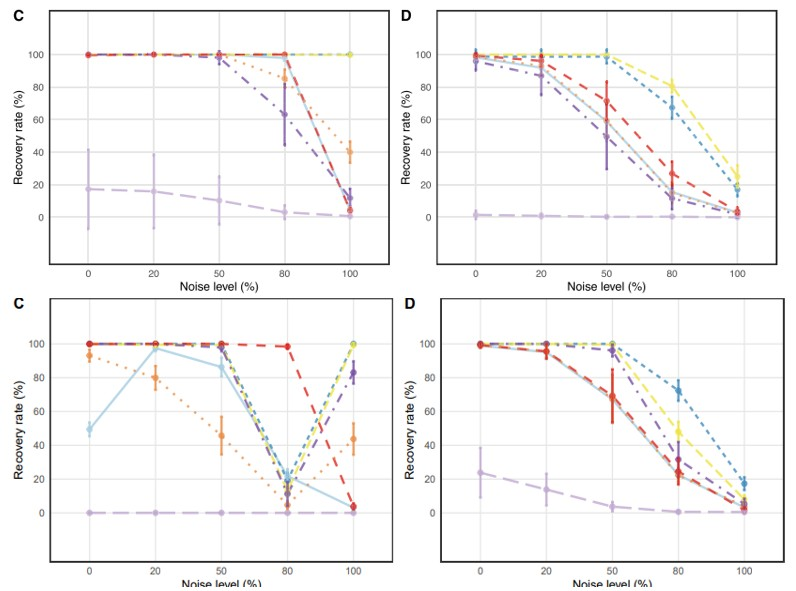
\includegraphics[width=0.9\linewidth]{Figure/noise_zero.jpg}
		\end{figure}
	\end{frame}
	
	

	\begin{frame}{The sensitivity and false-positive rate of scGSA performance}
		\begin{figure}[h!]
			\centering
			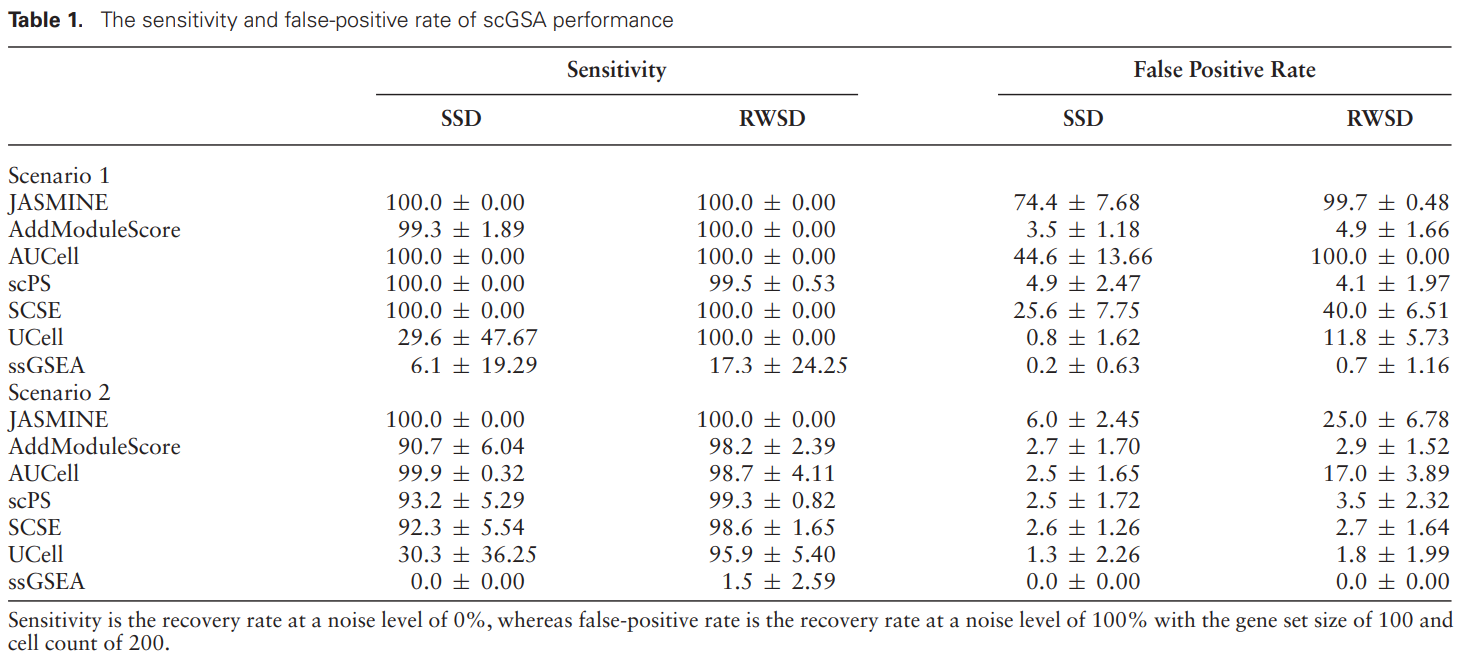
\includegraphics[width=\linewidth]{Figure/rate.png}
		\end{figure}
	\end{frame}
	
	\begin{frame}{The sensitivity and false-positive rate of scGSA performance}
		\begin{enumerate}
			\item This increased detection of false-positive gene sets by JASMINE and AUCell can be attributed to their reliance on gene expression rank without accounting for the magnitude of changes.
			\item scPS and AddModuleScore return a few false-positive gene sets at a 100$\%$ noise level in data with and without zero imputation, which increases their accuracy and reliability.
		\end{enumerate}
	\end{frame}

	\begin{frame}{Effect of the condition-specific genes }
		\begin{figure}[h!]
			\centering
			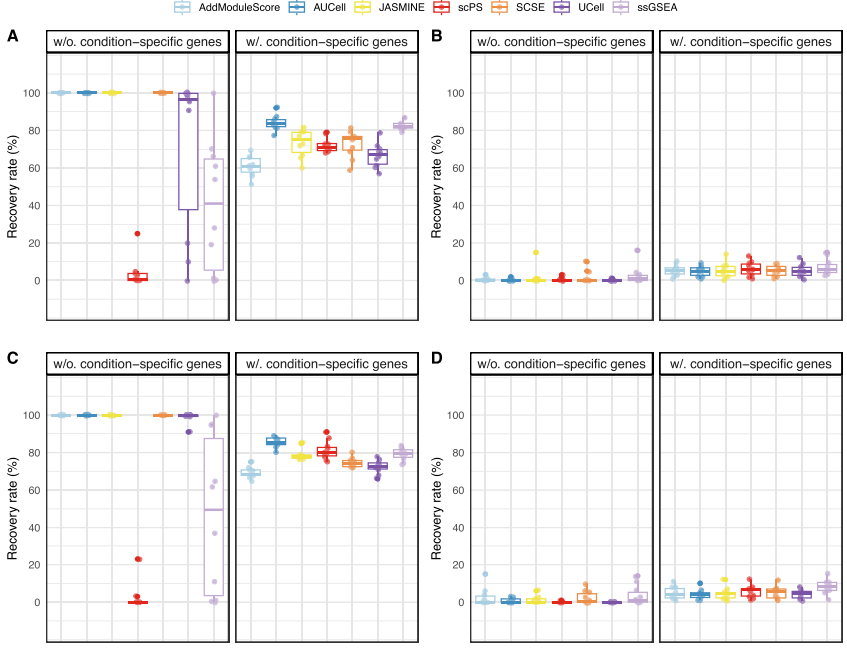
\includegraphics[width=0.75\linewidth]{Figure/condition.png}
		\end{figure}
	\end{frame}

\end{document}
